% ======================= Pre-Amble =========================
      
%Format
\documentclass[11pt, oneside]{article}   	% use "amsart" instead of "article" for AMSLaTeX format 
                     						%imports package {article} and specify option(s) [11pt, oneside]
\usepackage{geometry}                		% See geometry.pdf to learn the layout options. There are lots. 
    \geometry{letterpaper}                   		% ... or a4paper or a5paper or ... 
    %\geometry{landscape}                		% Activate for rotated page geometry

\usepackage[parfill]{parskip}    		        % Activate to begin paragraphs with an empty line rather than an indent

    %Colours
    \usepackage{graphicx, subcaption}
    \usepackage[usenames, dvipsnames]{color}     % font colour:    \textcolor{<colour>}{text}
          									%highlight text:  \colorbox{<color>}{text}
    \usepackage{soul}						%highlight text: \hl{}     %only  yellow								
    									%list of colours: https://www.sharelatex.com/learn/Using_colours_in_LaTeX
    									
    %Bullets
    \usepackage{enumerate}     %specify type of enumeration: \being{enumerate}[<type of enumeration>]
    
    %Footnote Spacing
    \setlength{\footnotesep}{0.4cm}                  %specify spacing b/w footnotes
    \setlength{\skip\footins}{0.6cm}                    % space b/w footnotes and textbody

	%Sections
%	\makeatletter
%	% we use \prefix@<level> only if it is defined
%	\renewcommand{\@seccntformat}[1]{
%	  \ifcsname prefix@#1\endcsname
%	    \csname prefix@#1\endcsname
%	  \else
%	    \csname the#1\endcsname\quad 
%	  \fi}
%	% define \prefix@section
%	\newcommand\prefix@section{Question \thesection}
%	\makeatother

%	\makeatletter
%	\def\@seccntformat#1{%
%	  \expandafter\ifx\csname c@#1\endcsname\c@section
%	  Question \thesection
%	  \else
%	  \csname the#1\endcsname\quad
%	  \fi}
%	\makeatother



%Mattematics
    %American Mathematics Society packages
    \usepackage{amsmath}	   %math
    \usepackage{amssymb}       %symbols
    \usepackage{amsthm}          %theorems
    \newtheorem{proposition}{Proposition}

    %QED
    \newcommand*{\QEDA}{\hfill\ensuremath{\blacksquare}}         %make qed filled square:    \QEDA
    \newcommand*{\QEDB}{\hfill\ensuremath{\square}}               %make qed empty square: \QEDB 
    \renewcommand\qedsymbol{\ensuremath{\blacksquare}}		%Proof environment
    
    % Proofs
	\newtheorem{thm}{Theorem}[section]
	\newtheorem{lem}[thm]{Lemma}
	\newtheorem{prop}[thm]{Proposition}
	\newtheorem*{cor}{Corollary}
	
	\theoremstyle{definition}
	\newtheorem{defn}{Definition}[section]
	\newtheorem{conj}{Conjecture}[section]
	\newtheorem{exmp}{Example}[section]
	
	\theoremstyle{remark}
	\newtheorem*{rem}{Remark}
	\newtheorem*{note}{Note}
	
	% Symbol Shortcuts
	\newcommand{\R}{\ensuremath{\mathbb{R}}}
	\newcommand{\C}{\ensuremath{\mathbb{C}}}
	\newcommand{\Z}{\ensuremath{\mathbb{Z}}}
	\newcommand{\Q}{\mathbb{Q}}
	\newcommand{\N}{\mathbb{N}}
	
	% Augmented Matrix
	\makeatletter
	\renewcommand*\env@matrix[1][*\c@MaxMatrixCols c]{%
  	\hskip -\arraycolsep
 		 \let\@ifnextchar\new@ifnextchar
 		 \array{#1}}
	\makeatother
	
    %\numberwithin{counterA}{counterB} 	% replaces counterA by counterb.countera
	%\numberwithin{equation}{question} 	% for equations: (5) -> (6.1)
    
    % Spacing Units
	\usepackage{siunitx}				% Syntax: \SI{value}{unit}
								%	-> e.g. $\SI{-9.81}{ms^{-2}}$
	
    % MATLAB in sentence (need mcode.sty in folder)
	%\usepackage[]{mcode} % http://www.mathworks.com/matlabcentral/fileexchange/8015-m-code-latex-package
	% Syntax:
	%	- In Sentence: \mcode{<code>}
	%	- Block of code: \begin{lstlisting} <code> \end{lstlisting}
	%	- Footnote: \footnote{ \mcodefn{ <code> } }
	%	- External m-file
	%		-> Entire file: \lstinputlisting{/SOME/PATH/FILENAME.M}
	%		-> Certain lines (i.e. skip header): \lstinputlisting[firstline=6, lastline=15]{/SOME/PATH/FILENAME.M}



%Figures
\usepackage{caption}
\captionsetup[figure]{labelfont=bf}    %make figure labels boldface
\captionsetup[table]{labelfont=bf}     %make table labels boldface

\usepackage[hidelinks]{hyperref}                % Allows for clickable references

    %Tables
    \usepackage[none]{hyphenat}                    % Stops breaking-up words in a table (i.e. no hyphens)                                                             
    
    \usepackage{array}   
        \newcolumntype{x}[1]{>{\centering\let\newline\\\arraybackslash\hspace{0pt}}p{#1}}       %center fixed column width: x{<len>}                      
        \newcolumntype{$}{>{\global\let\currentrowstyle\relax}}                                 % let us apply things (e.g. bold/italicize) to entire row            
        \newcolumntype{^}{>{\currentrowstyle}}
        \newcommand{\rowstyle}[1]{\gdef\currentrowstyle{#1} #1\ignorespaces}
    
    %Images
    \graphicspath{ {images/} }                          %directory that your images are located in within your current directory
    
    %Diagrams
    \usepackage[latin1]{inputenc}
    \usepackage{tikz}
    	\tikzset{line/.style={-latex'}}
        \usepackage{tkz-berge}
        \usetikzlibrary{shapes,arrows}
        \usetikzlibrary{patterns}			%Specify colours of stuff (e.g. vertices): 
        										%	-> set style: \tikzset{VertexStyle/.append style = {minimum size = 8pt, inner sep = 0pt}} 
											%	-> change individual vertices: \AddVertexColor{white}{1,2} 
%Bibliography
\usepackage[numbers,sort&compress]{natbib}   %for multiple references: sorts  (i.e. [1,2] NOT [2, 1] )
                                           				  %                                     compresses (i.e. [1-3] )
\usepackage[nottoc]{tocbibind}                            %add bibliography to table of contents

%Miscellaneous 
\usepackage{wasysym} 	 % \smiley{} \frownie{} \blacksmiley{}
\usepackage{hyperref}
\usepackage{algpseudocode}


%================================== Header & Footer =======================================
\usepackage{fancyhdr}
\usepackage{lastpage}      %ensures you can reference LastPage (i.e. Page 2 of 10)
\renewcommand{\headrulewidth}{0.4pt}		%Decorative Header line: thickness={0.4pt}
\renewcommand{\footrulewidth}{0.4pt}		%Decorative Footer line: thickness={0.4pt}
\setlength{\headheight}{13.6pt} 		%space b/w top of page & header
\setlength{\headsep}{0.3in}		%space b/w page header and body
%Make Header & Footer    
\pagestyle{fancy}
    \lhead{S. Knill and T. Darra} 		% controls the left corner of the header
    \chead{} 					% controls the center of the header
    \rhead{} 					% controls the right corner of the header
    \lfoot{} 					% controls the left corner of the footer
    \cfoot{Page~\thepage\ of \pageref{LastPage}} 				% controls the center of the footer
    												%Page~\thepage\  if just want Page x
    \rfoot{}			 		% controls the right corner of the footer
% ================================== Document =============================================
\begin{document}
% Implementation of a Database Management System for The Dempster Carte
\title{CPSC 320 -- Assignment 2
\line(1,0){360} \\               %(slope x, y){length of line}
\vspace{0.5cm}
\large
The University of British Columbia \\
Due: October 6, 2016
\vspace{1cm}}
\author{
Knill, Stephanie\\
54882113
\and
Darra, Taj \\
43350115
}
\date{}                    % Activate:  display a given date (e.g. {August 4} ) or no date (empty {} )
                                    %No activate: display current date
\maketitle
\thispagestyle{empty}    %do not display page number on this page

\medskip 
\section*{Collaboration Policy}
\emph{All group members have read and followed the guidelines for academic conduct in CPSC 320. As part of those rules, when collaborating with anyone outside my group, (1) I and my collaborators took no record but names away, and (2) after a suitable break, my group created the assignment I am submitting without help from anyone other than the course staff.}

% ================= Questions ================
\cleardoublepage
\section{Olympic Scheduling}
\textit{You are in charge of a live-streaming YouTube channel for the Olympics that promises never to interrupt an event. (So, once you start playing an event, you must play only that event from the time it starts to the time it finishes.) You have a list of the events, where each event includes its: \textbf{start time, finish time (which must be after its start time), and expected audience value}. Your goal is to \textbf{make a schedule to broadcast the most valuable complete events}. \textbf{The best schedule is the one with the highest-valued event}; \textbf{in case of ties, compare second highest valued events, and so on}. (So, for example, you obviously \textbf{will} include the single highest-valued event in the Olympics---presumably the hockey gold medal game---no matter what else it blocks you from showing.) (Times when you're not broadcasting events will be filled with ``human interest stories'' that have zero value; so, they're irrelevant.) \textbf{ASSUME: all event values are distinct and all event times are distinct.} I.e., for any two values $v_i$ and $v_j$ with $i \neq j$, $v_i \neq v_j$. The same holds for start and end times (e.g., for any two start times $s_i$ and $s_j$ with $i \neq j$, $s_i \neq s_j$). Further, for any two start and finish times $s_i$ and $f_j$,
whether $i = j$ or not, $s_i \neq f_j$.}

\subsection{Na\"ive Algorithm}
\textit{Consider the following algorithm. Assume that deleting an event from a list of events takes constant time.}
\begin{verbatim}
Naive(E):
  result = new empty list of events
  while E is not empty:
    bestEvent = E[0]
    for each e in E:
      if value(e) > value(bestEvent):
        bestEvent = e
    delete bestEvent from E
    for each e in E:
      if start(e) < finish(bestEvent) and finish(e) > start(bestEvent):
        delete e from E
    add bestEvent to result
  return result
\end{verbatim}

\subsubsection{Finiteness}
\textit{Briefly sketch a proof that the \texttt{while} loop in the algorithm above terminates. You need not give a formal proof, but you should include all key insights in the proof.}

\textbf{Representing the problem:} Let $E$ denote the set of all events to be streamed $E=\left\{e_1, \ldots, e_n\right\}$. For every event $e \in E$, let $e$ comprise an ordered triple $e_i = (v_i, s_i, f_i)$ where $v,s$ and $f$ denote the audience value, start time, and finish time accordingly.

\begin{proof}
Let $n$ be the cardinality of $E$ (i.e. $n=|E|$).

\textbf{Base Case:} if $n = 0$, then the while loop is never intiated.
Otherwise if $n=1$ then the event $e \in E$ is the bestEvent and is removed after the execution of the first for loop. 

\textbf{Inductive Step:} Assume true for $n=k$ events, then for $n=k+1$ events we have two cases as such:
\begin{itemize}
	\item In the first case, we delete the bestEvent and no conflicting events, which leaves us with $n=k+1-1=k$. By the inductive assumption the algorithm holds true.
	\item As for the second case, we delete the bestEvent and some number of events which leaves u with $n<k$. Again by the inductive step, the algorithm holds true.
\end{itemize} 
\end{proof}

\subsubsection{Efficiency}
\textit{Give and briefly justify a good asymptotic bound on the runtime of the algorithm.}

Assuming all elementary operation execute in constant time, the worst case executes in $O(n^2)$ time, where the worst case execution is defined as when we only delete the assigned bestEvent (i.e. there are no conflicts). 

Here the while loop executes a total of $n$ times. Within each execution of the while loop, we have the first for loop, deletion of bestEvent (constant time), the second for loop, and the addition of bestEvent (constant time). The first for loop executes $n$ times for comparing the values of bestEvent and another event $e$; the second for loop executes for $(n-1)$ iterations. In total, we have: $$n \cdot (n + (n-1)) = O(n^2)$$

\subsubsection{Correctness}
\textit{Briefly sketch a proof that the algorithm is correct. You need not give a formal proof, but you should include all key insights in the
proof.}

\textbf{Correctness:} Let us define a correct solution returned by the algorithm as a set $R \subseteq E$. For $R=\{r_1, r_2, \ldots, r_k\}$, we have that $v_1 > v_2 > \ldots > v_k$. To prevent conflicted showtimes of events we have $ \forall r_i, r_j \in R, \text{if } s_i < s_j, \text{then } f_i < s_j$; or less formally, if an event in our schedule $R$ begins before the next event, then it will also end before the start of our next event.

\begin{proof}
	We will show that the \texttt{Naive}($E$) algorithm returns a correct solution but not necessarily the optimal solution. If we can show that (1) the bestEvent (i.e. $e_i\in E$ such that $v_i$ is a max) is removed from $E$ and added to our result $R$, (2) all conflicting events to bestEvent are removed from $E$, and (3) the algorithm repeats steps (1) and (2) for all remaing events in $E$, then we have shown \texttt{Naive}($E$) returns a correct solution. 
	\begin{enumerate}
		\item The bestEvent $e_\text{best}$ is initially assigned as the first element of $E$, then the value of the bestEvent is compared to the value of another element, $e_\text{other}$ . If $v_\text{other} > v_\text{best}$ then we assign the bestEvent $e_\text{best} = e_\text{other}$. Hence, $v_\text{best}$ is the maximum audience value in $E$.
		
		After the execution of the first for loop, we remove the bestEvent from $E$ and regardless of the execution of the second for loop this bestEvent is added to $R$.
		
		\item In order to handle the conflicts, the second for loop removes events that satisfy the following condition: for all $ e_i \in E - \{e_\text{best}\}$ if an event $e_i$ has a start time before or during the bestEvent (i.e. $s_i < f_\text{best}$), and the finish time of $e_i$ is during or after the bestEvent (i.e. $f_i > s_\text{best}$), then the event $e_i$ interrupts the bestEvent. To see why, let us break the start time of $e_i$ into two cases.
		
			\textbf{Case 1:} event $e_i$ starts before the bestEvent. If $e_i$ ends after the start of the bestEvent (i.e. the second condition $f_i > s_\text{best}$), then we have an overlap.
		
			\textbf{Case 2}: event $e_i$ starts during the bestEvent. By definition, we have an overlap.
		
		\item After steps (1) and (2) we are now left with the subset $E' \subset E$, such that $E'$ does not contain the bestEvent (1) and any conflicting events (2). According to the while loop, if $E'$ is non-empty, then the algorithm will repeat steps (1) and (2) for this new $E'$.
	\end{enumerate}
\end{proof}

\subsection{Reduction on Simplified Problem}
\textit{To make the Olympic Broadcasting problem simpler, we completely remove start time and finish times from the problem. So, now events only have values (not times), and a ``schedule'' is just a set of selected events. To make it slightly harder again, you are not allowed to select two events $i$ and $j$ if their values are within 10 units of each other: $|v_i - v_j| \leq 10$. Give a correct reduction from this simplified Olympic Broadcasting problem to the sorting problem (where you provide both a list of items and a function to compare two items). Your reduction should take $O(n \lg n)$ time.}

\textit{\textbf{NOTE:} You will likely find that (a) you can solve this with a single call to the sorting problem's solution algorithm and (b) producing the sorting instance is the easier part and transforming the solution to sorting into a solution to this simplified Olympic Broadcasting problem is the harder part. Don't forget to do both!}

\textbf{Reduction:} Let us first sort our events $E$ in descending order of value, which will be stored in $H$ (i.e. for all events $e \in H$,  $v_1 > v_2 > \dotsm> v_n$ where $n =|H|$). To make this an $O(n \lg n)$ operation, we will store the data as a max heap $H = \texttt{Heapify}(E)$,

For our comparaison function, we want to know if we can add an event $e_j$ if we have already added an event $e_i$. The pseudocode is given below.
\begin{verbatim}
	canAdd(e_i, e_j):
	  if |value(e_i) - value(e_j)| > 10
	    return true
	  else
	    return false	
\end{verbatim} 

Using our sorting algorithm and comparison function, we can now define an algorithm to reduce our simplified Olympic Broadcasting problem:
\begin{verbatim}
  Reduction_Simplified(E):
    H := Heapify(E)    
    result := new empty list of events
    prev := H[0]	            // add highest value event to result
    delete prev from H
    add prev to result
    
    while H is not empty:
      if canAdd(prev, H[0]):
        add H[0] to result
      prev := H[0]
      delete prev from H
      
    return result 
\end{verbatim}


\subsection{Olympic Reduction, BONUS ONLY}
\textit{This was significantly harder than we intended it to be! So, we removed it from the quiz/assignment. It's a bonus problem worth two CPSC 320 bonus points for extremely clear, correct, and efficient responses. (Extremely clear reductions that take $O(n)$ time---not counting an $O(1)$ number of calls to a sorting algorithm---may receive 3 bonus points, but we don't know if such reductions are possible.) Give a correct and efficient reduction from the Olympic broadcasting problem to the sorting problem (where you provide both a list of items and a function to compare two items). Your reduction---combined with an $O(n \lg n)$ sorting algorithm---should be asymptotically more efficient than the na\"ive algorithm above.}

%Let us first modify our comparison function, \texttt{canAdd}. From the given Na\"ve algorithm in 1.1, we know that criteria for overlap is given by 
%$$\text{start}(e) < \text{finish}(\text{bestEvent}) \text{ and finish}(e) > \text{start}(\text{bestEvent})$$
%Adapting this to our \texttt{canAdd} algorithm, we can define it as
%\begin{verbatim}
%  canAdd(e_i, e_j):
%    if !(start(e_j) < finish(e_i) and finish(e_j) > start(e_i))
%      return true
%    else
%      return false	
%\end{verbatim}
%
%Although our psuedocode algorithm in 1.2 is sufficiently abstract, we now have a problem with how our algorithm checks if we can add the next event. In the simplified model, we only needed to check the most recently added event to \texttt{result}. However, in our more realistic model where all events have start and end times, we need to check \emph{all} of the added events in \texttt{result}---we need to ensure that the new event does not overlap with any of the already added higher valued events. With a slight modification to our algorithm, we have
%
%\cleardoublepage
%\begin{verbatim}
%  Reduction(E):
%    H := Heapify(E)    
%    result := new empty list of events
%    
%    while H is not empty:
%      
%      // Check if canAdd for all events r in result
%      valid := true;
%      for all r in result
%        if ! canAdd(r, H[0]):
%          valid := false
%          break
%      
%      // add H[0] if valid
%      if valid      
%        add H[0] to result  
%      
%      // Regardless if added, remove H[0]
%      delete H[0] from H
%    
%    return result 
%\end{verbatim}

\subsubsection{Correctness}
\textit{Briefly sketch a proof that your algorithm is correct. You need not give a formal proof, but you should include all key insights in the proof.}

%\begin{proof}
%	Let us first show that our \texttt{canAdd} comparison function is correct. By our proof of Correctness in Section 1.1.3, we know that the criteria for overlap is indeed $\text{start}(e) < \text{finish}(\text{bestEvent}) \text{ and finish}(e) > \text{start}(\text{bestEvent})$. Since we know when we \textit{cannot} add another event $_j$ if we have already added $e_i$, then the negation of it will tell us when we \textit{can}.
%	
%	Now we will prove that our algorithm psuedocode is correct. As aforementioned, we need to check \emph{all} of the added events in \texttt{result} before we can add our next highest valued event $H[0]$. This is accomplished by checking if \texttt{canAdd}($r, H[0]$) is true for all events $r$ in our result $R$. If it is, we will add the next highest event $H[0]$ to $R$ (if not, no addition is done). Regarless if the addition is carried out, however, we remove $H[0]$ from our max heap $H$ and reheapify. Thus we will attempt to add each event in $H$ in decreasing order of value and we will make progress to our termination case $H=\emptyset$.
%\end{proof}

\subsubsection{Efficiency}
\textit{Give and briefly justify a good asymptotic bound on the runtime of \textbf{just} your reduction, \textbf{not} including the call to the sorting algorithm. So, for the purposes of this asymptotic bound, you can imagine that we somehow solve sorting in constant time. (Note: it's possible to give a reduction that takes $O(n)$ time.)}

%Assuming by some miriacle that our calls to heap sort (i.e. our initial call to Heapify $E$ and to reheapify upon deletion of $H[0]$) and all other operations can be done in constant time, then we only need to examine our barometer function, the for loop. In the worst case, we add all events in $H$ to $R$. Thus in the first iteration $|R|=1$, in the second iteration we have $|R|=2$, and so on. Thus we have a total of
%
%$$1+2+\ldots + (n-1) = \frac{n(n-1)}{2}$$
%
%iterations, or $O(n^2)$ assymptotic runtime.

\cleardoublepage
\section{Exhausted of Marriage}
\textit{We modify SMP with the very reasonable change that not every woman need list every man in her preferences. She prefers to be unmarried to marrying unlisted men. Note that she clearly prefers any man on her
preference list to any man not on her preference list. Men can similarly truncate their lists of women. Here is the Gale-Shapley algorithm:}
  \begin{algorithmic}[1]
  \Procedure{Stable-Marriage}{$M$, $W$}
    \State initialize all men in $M$ and women in $W$ to unengaged
    \While {an unengaged man with at least one woman on his preference list remains}
      \State choose such a man $m \in M$
      \State propose to the next woman $w \in W$ on his preference list
      \If {$w$ is unengaged}
        \State engage $m$ to $w$
      \ElsIf {$w$ prefers $m$ to her fianc\'e $m'$}
        \State break engagement of $m'$ to $w$
        \State engage $m$ to $w$
      \EndIf
      \State cross $w$ off $m$'s preference list
    \EndWhile
    \State report the set of engaged pairs as the final matching
  \EndProcedure
  \end{algorithmic}
\textit{With one small change, we can apply this algorithm and ensure that the (not necessarily perfect) matching produced never marries a person to someone they left off of their preference list.}

\begin{enumerate}
	\item \textit{Make the small change necessary \textbf{to the algorithm above}.}
	
	\qquad Line 6: if ($w$ is unengaged \& $m$ in $w$'s preference list) then
	\item \textit{Briefly sketch the key elements of a proof that the algorithm terminates.}
	
	In the worst case, the algorithm will terminate in $n^2$ iterations, i.e. men have complete preference lists. Let $S(k)$ be the set of pairs $(m, w)$ such that $m$ has proposed to $w$ on iteration $k$ of the Gale-Shapley algorithm. Then we can see that every new iteration increases the number of pairs (or in mathematical notation: $\forall k, |S(k+1)| > S(k)$). However, since in the worst case we have $n^2$ possible pairs of men and women we know that there can be at most $n^2$ iterations of the while loop, hence the algorithm must terminate.
	
	
	\item \textit{We need a new definition of instability now that some people may end up unmarried. Here is one new type of instability that we call an \emph{elopement instability}: m$_i$ and w$_j$ are both unmarried but list each other on their preference lists (in which case they have incentive to break the imposed matching and marry each other).}
   
   \textit{Describe another new type of instability involving an unmarried woman. (Note: an analogous instability exists involving an unmarried man.)}
   
   \textbf{The mistress instability:} We can define a new instability with the following conditions:
   		\begin{enumerate}
   			\item $w_j$ is unmarried, $m_i$ is married
   			\item $w_j$ prefers $m_i$ to being unmarried 
   			\item $m_i$ prefers $w_j$ to current partner
   
   \end{enumerate}
   \textbf{The poolboy instability} \textit{(to be referenced in 2.1)}: An instability analogous to the above has the following conditions: 
   \begin{enumerate}
   			\item $w_j$ is married, $m_i$ is unmarried
   			\item $w_j$ prefers $m_i$ to current partner
   			\item $m_i$ prefers $w_j$ to being unmarried
   
   \end{enumerate}
	\item \textit{Briefly sketch the key elements of a proof that your modified G-S algorithm cannot generate an elopement instability.}
	
	\begin{proof}
		In order to show that the \textit{elopement instability} is not a feasible result of the modified G-S algorithm, we will show that the algorithm always terminates with all men either left married or unmarried with an empty preference list. The precondition of the \textbf{while} loop outlines that an unengaged man must have a preference list, otherwise we terminate the procedure. This means that we cannot have an unengaged man and unengaged woman that prefer each other. This is because the while loop ensures that every man gets engaged or is left with an empty preference list. In the case of the latter, it is not possible that an unmarried man prefers any woman.
	\end{proof}
\end{enumerate}

\subsection{Even More Exhausted}
\textit{Briefly sketch the key elements of a proof that your modified G-S
algorithm cannot generate any of the other three types of instability
(the classic SMP instability, the instability you defined above, and
the analogous instability with the roles of men and women swapped).}

\begin{proof}
To show that no such instability may arise, we will construct a mini ``proof" for each instability.

\begin{enumerate}
	\item \textbf{No Classic SMP Instability}
	
	Let us reduce our problem to that of a classic SMP, which does not have a classic SMP instabilty. To convert to a classic SMP, we will add men/woman to the preference lists of our modified SMP in order to make them full (i.e. if $n=4$ and $w$ has preference list $\{m_2, m_4\}$, then her new preference list will be $\{m_2, m_4, m_1, m_3\}$). Running the G-S algorithm gives us the same matching as the modified G-S algorithm, except the oriignally unmarried men and women (if any) are now paired up with each other. Thus the solution set of married pairs of our modified SMP $S_\text{modified}$ can be viewed as a subset of the solution of the classic SMP $S_\text{classic}$, or in mathematical notation $S_\text{modified} \subseteq S_\text{classic}$. Since $S_\text{classic}$ does not have classic SMP instabilities and $S_\text{modified}$ is a subset, then  $S_\text{modified}$ also does not have a classic SMP instability.

	\item \textbf{No Mistress Instability}
	
	Assume to the contrary that for an unmarried woman $w$ and married man $m$, we have that (1) $w$ prefers $m$ to being unmarried (i.e. $m$ is on $w$'s preference list) and (2) $m$ prefers woman $w$ to his current partner $w'$. This means that $m$ proposed to $w$ before $w'$. However, we know that $w$ is unmarried and $m$ is on her preference list. This gives us the necessary contradiction as a woman cannot break an engagement in favour of being unmarried or reject a man on her preference list if she is unmarried.

	\item \textbf{No Poolboy Instability}
	
	For the Poolboy Instability to arise, there must exist an unmarried man that has a non-empty preference list by conditions (a) and (c). As shown above in proof 2.1.4, the modified G-S algorithm terminates with all men either married or unmarried with an empty preference list, thereby making this instability impossible.
	
\end{enumerate}
\end{proof}



\cleardoublepage
\section{Footblog}
\textit{The massive social network Footblog tracks relationships based on
whether two people have ``enemied'' each other. (``Enemyship'' is a mutual agreement, meaning that a person is not allowed to ``enemy'' another person unless the other person agrees to ``enemy'' them back. No one can ``enemy'' themselves.)}

\subsection{Isolationism}
\textit{We investigate whether Footblog's network is a single connected
component. Footblog's founder created the first Footblog account, and that account has no ``sponsor'' (and cannot be assigned one). Every other account must have a single, designated ``sponsor'' who they have ``enemied''. If $a$ sponsors $b$, we call $b$ the\emph{sponsee} of $a$. There are then four major actions to consider on Footblog, some of which involve others as steps:}
\begin{description}
	\item[\emph{Joining}] When a new Footblog member joins, they must do so by
               choosing as sponsor (and ``enemying'') someone already in
               the network who agrees to be their sponsor (and their
               enemy). After members join, they're free to ``enemy''
               and ``unenemy'' anyone except their sponsor and their
               sponsees.
	\item[\emph{Enemying}] Already described above. Remember that when one person
                ``enemies'' another, the other must agree to ``enemy''
                that person back.
	\item[\emph{Un-Enemying}] Unlike making an ``enemy'' link, one person alone can
                   ``unenemy'' another person, in which case neither
                   ``enemies'' the other any more.
	\item[\emph{Change Sponsor}] If a person wishes to change their sponsor, they
     must ``unenemy'' their sponsor and simultaneously ``enemy'' a new
     sponsor. The new sponsor must agree to act as sponsor and enemy
     and \textbf{must be a new enemy} (i.e., must not already be the person's
     enemy). Note that while a sponsee can choose to change their
     sponsor, a sponsor cannot choose to change their sponsee.
\end{description}
\textit{You may assume these actions never happen in parallel, i.e., a defined sequence occurs of the operations: joining, enemying, un-enemying, and changing sponsors.}
\begin{enumerate}
	\item \textit{Based on these rules, sketch a brief proof that when a person changes their sponsor, their new sponsor cannot also be one of their sponsees.}
	
	\begin{proof}
		Assume to the contrary that for a person $p$ their new sponsor $s$ is also their sponsee. Since $s$ was originally a sponsee, then $p$ and $s$ were already enemies. However this contradicts the definition of ``Change Sponsor'', as the new sponsor must be a new enemy.
	\end{proof}		
	
	\item \textit{Based on these rules, either \textbf{sketch the key points in a proof that    Footblog's enemy graph forms a single connected component} or \textbf{give a small sequence of actions that creates multiple components}.}
   
   Circle \textbf{one}: \hfill \textbf{SINGLE ONLY} \hfill \textbf{MAY BE MULTIPLE} \hfill
   \textbf{Provide your proof sketch or example:}
   
   Let the creator be denoted by the vertex $C$. Then a sequence of steps that will generate multiple components is
   \begin{verbatim}
     join(A, C)
     join(B, A)
     join(D, B)
     changeSponsor(A, D)
   \end{verbatim}
   where join($v_i$, $v_j$) adds the vertex $v_i$ to the network with $v_j$ as its sponsor and changeSponsor($v_i$, $v_j$) changes the sponsor of vertex $v_i$ to be $v_j$.
   
   
   To help visualize these steps, let us represent it as a graph $G=(V,E)$ such that an edge $(v_i, v_j)$ is defined if $v_i$ and $v_j$ are enemies. For ease of clarity, we will show a sponsor-sponsee relationship by a directed arrow, where the arrow head points to the sponsor. The graph $G$ prior to the call to changeSponsor is shown in Figure \ref{Graph1} and the graph $G'$ after the call to changeSponsor in Figure \ref{Graph2}.
   
   \begin{figure}[h]           
   	\centering
    \begin{subfigure}[b]{0.45\columnwidth}
    		\centering
        \begin{tikzpicture}[scale=0.75,transform shape]
              \tikzstyle{LabelStyle}=[fill=white,sloped]
              \Vertex[x=0,y=0]{B}
              \Vertex[x=0,y=3]{A}
              \Vertex[x=3,y=0]{D}
              \Vertex[x=3,y=3]{C}
            
              %Edges bend left
              \tikzstyle{EdgeStyle}=[bend left]		%\Edge[label=$120$](A)(B)  %if want to label the edge
                  			
              %Edges bend right
              \tikzstyle{EdgeStyle}=[bend right]
            
              %Edges arrow
              \tikzstyle{EdgeStyle}=[->]
                  \Edge(A)(C)
                  \Edge(B)(A)
                  \Edge(D)(B) 
         \end{tikzpicture}
         \caption{Graph $G$}
		 \label{Graph1}
    \end{subfigure}
    \begin{subfigure}[b]{0.45\columnwidth}
    		\centering
        \begin{tikzpicture}[scale=0.75,transform shape]
              \tikzstyle{LabelStyle}=[fill=white,sloped]
              \Vertex[x=0,y=0]{B}
              \Vertex[x=0,y=3]{A}
              \Vertex[x=3,y=0]{D}
              \Vertex[x=3,y=3]{C}
            
              %Edges bend left
              \tikzstyle{EdgeStyle}=[bend left]		%\Edge[label=$120$](A)(B)  %if want to label the edge
                  			
              %Edges bend right
              \tikzstyle{EdgeStyle}=[bend right]
        
              %Edges arrow
              \tikzstyle{EdgeStyle}=[->]
                  \Edge(A)(D)
                  \Edge(B)(A)
                  \Edge(D)(B) 
         \end{tikzpicture}
         \caption{Graph $G'$}
		 \label{Graph2}
    \end{subfigure}
    \caption{A simply connected Footblog graph $G$ and the same graph $G'$ after changeSponsor is called.}
    \label{polynomials}
	\end{figure}
   
\end{enumerate}
\subsection{Centrality}
\textit{Footblog has defined a notion of ``centrality'' for its users: a user's ``centrality'' is the minimum number of people they'd need to go through to get a message to the person farthest from them on the network, following ``enemy'' links. (The ``farthest'' person is exactly the one to whom there is the longest minimum-length path of enemies.) For this problem, \textbf{assume that the Footblog network does indeed form a single connected component.} Briefly describe an algorithm to compute the centrality of a userngiven a graph $G$ represented as a number of users $n > 0$ (where the users themselves are vertices named $\{v_1, v_2, \ldots, v_n\}$, a vertex number $i$ (where $1 \leq i \leq n$) of the user whose centrality we wish to compute, and an adjacency list $A$ of edges (i.e., an array of linked lists, where the entries in the list $A[j]$ are the vertex numbers of the users $j$ has ``enemied''). You may use any common data structures you need. \textbf{Your algorithm must run in linear (i.e., $O(n + m)$ for $n$ nodes and $m$ edges) time.}}
\begin{verbatim}
Centrality(n, i, A):
  // Initialize distances
  V := set of all vertices in graph G
  for each vertx v in V - {v_i}
    dist[v] := infinity
  dist[i] := 0
  
  // Modified Dijkstra algorithm: compute shortest distance between
  // v_i and all other vertices
  while V is not empty:
    u: node in V with smallest dist[]
    remove u from V
    
    for each v in A[u]		   // all of u's neighbours
      temp := dist[u] + 1
      if temp < dist[v]
        dist[v] := temp
  
  // Find maximium of the shortest distances
  max_dist = 0
  for each vertex v in V:
    if dist[v] > max_dist
      max_dist := dist[v]
    
  return max_dist
\end{verbatim}
\textbf{Runtime Analysis:} since the initialization of distances is done over $n$ vertices and the modified Dijkstra algorithm runs over $m$ edges, we have $O(n+m)$.


\cleardoublepage
\section{Heaps of Fun Might Be OK}
\textit{You're managing a major online tournament of the hot new game Flappy
Squirrel. There are a huge number of users, each with a
competitiveness rating (a floating point number). You need an
algorithm that---given a desired number of competitors $c$ and a list
of these competitiveness ratings (an array $A$ of length
$n$)---returns a list of the $c$ highest ratings. You're guaranteed
that $c \leq n$. (Note: we use 1-based indexing on arrays.)}

\subsection{Algorithm 1}
\textit{Give and briefly justify a good asymptotic upper-bound (i.e., big-$O$
bound) on the runtime of the following algorithm to solve this problem. (\textbf{Note:} the \texttt{buildMaxHeap} operation returns a max-heap built from the elements of a given array of length $n$ in $O(n)$}
time.)
\begin{verbatim}
TopC(A, c):
  best <- empty list
  h <- buildMaxHeap(A)
  for i = 1 to c:
    add findMax(h) to best
    deleteMax(h)
  return best
\end{verbatim}

\textbf{Answer: } The asymptotic upper-bound seems to be $O(cn)$. Given that \texttt{buildMaxHeap} operates at $O(n)$ we proceed to the \texttt{for} loop that executes $c$ times. In this loop, we call \texttt{deleteMax} which removes the maximum element in the heap and calls the necessary percolations to rebalance the heap. This should take $O(n)$. Hence, we have $n+1+c(1+n)+1 = O(cn)$.

\subsection{Algorithm 2}
\textit{Give and briefly justify a good asymptotic upper-bound (i.e., big-$O$
bound) on the runtime of the following algorithm to solve this problem. (Note: the notation \texttt{A[1..c]} produces a list of the elements \texttt{A[1], A[2], A[3], ..., A[c]} in $O(c)$ time.)}
\begin{verbatim}
TopC(A, c):
  for i = 1 to c:
    maxIndex = i
    for j = i+1 to n:
      if A[j] > A[maxIndex]:
        maxIndex = j
    max = A[maxIndex]
    A[maxIndex] = A[i]
    A[i] = max
  return A[1..c]
\end{verbatim}

\textbf{Answer: } Algorithm 2 executes in $O(cn)$ time. The outer \texttt{for} loop  performs $c$ operations. The nested \texttt{for} loop performs  approximately $n$ operations. Thus, by the end of algorithm we have $O(cn + c) = O(cn)$


\subsection{Algorithm 3}
\textit{Give and briefly justify a good asymptotic upper-bound (i.e., big-$O$
bound) on the runtime of the following algorithm to solve this problem.}
\begin{verbatim}
TopC(A, c):
  sort A using an efficient, comparison-based sorting algorithm
  return A[1..c]
\end{verbatim}

\textbf{Answer: } Using a QuickSort as our comparison-based sorting algorithm, it takes $O(n \lg n)$ to sort \texttt{A}. Then to \texttt{return A[1...c]} it takes $O(c)$. The upper bound is then $O(c+n \lg n)$.  


\subsection{Algorithm 4}
\textit{Give and briefly justify a good asymptotic upper-bound (i.e., big-$O$
bound) on the runtime of the following algorithm to solve this problem. (Note: \texttt{Elements(h)} produces all elements in the heap \texttt{h} in
constant time, but \texttt{h} can no longer be used after that point.)}
\begin{verbatim}
TopC(A, c):
  h <- empty min-heap
  for i = 1 to n:
    if Size(h) < c:
      Insert(h, A[i])
    else if A[i] > FindMin(h):
      DeleteMin(h)
      Insert(h, A[i])
  return Elements(h)
\end{verbatim}

\textbf{Answer: }Given that \texttt{Insert} operates in $O(\lg n)$, \texttt{FindMin} returns the minimum in constant time, and \texttt{DeleteMin} takes $O(n)$ to call the necssary percolations to re-heapify the array, the Algorithm operates in $O(n^2)$. The worst case runtime occurs when control is passed to the \texttt{else} statement, where we iterate $n$ times over $n+\lg n$ operations. 

\end{document} 
